\documentclass[a4paper, 10pt, final, garamond]{book}
\usepackage{cours-preambule}

\raggedbottom

\makeatletter
\renewcommand{\@chapapp}{Induction -- chapitre}
% \renewcommand\thechapter{1 et 2}
\makeatother

\begin{document}
\setcounter{chapter}{2}

\chapter{TD~: Lois de l'induction, induction de \textsc{Neumann}}
\section{Étude qualitative de l'induction}
\label{sec:indquali}
\begin{enumerate}
	\item Pour les quatre schémas ci-dessous, indiquer le signe de l'intensité
	      dans le circuit.
	      \begin{figure}[h]
		      \centering
		      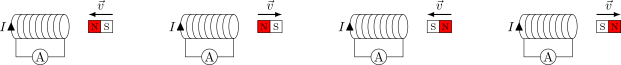
\includegraphics[scale=1]{indquali_a}
		      \label{fig:indquali_a}
	      \end{figure}
	\item En partant de la figure ci-dessous avec $\Sr_1$ et $\Sr_2$ deux
	      solénoïdes dont $\Sr_1$ est relié à un générateur et $\Sr_2$ à un
	      ampèremètre, répondre aux questions suivantes par «~vrai~» ou «~faux~» en
	      justifiant.
	      \begin{figure}[h]
		      \centering
		      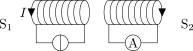
\includegraphics[scale=1]{indquali_b}
		      \label{fig:indquali_b}
	      \end{figure}
	      \begin{enumerate}
		      \item Le courant $I$ dans $\Sr_1$ étant constant, un courant circule dans
		            $\Sr_2$ dans le sens indiqué sur la figure.
		      \item Un courant circule dans $\Sr_2$ dans le sens indiqué lorsque $I$
		            augmente.
		      \item Un courant circule dans $\Sr_2$ dans le sens indiqué lorsqu'on
		            éloigne $\Sr_2$ de $\Sr_1$.
		      \item Un courant circule dans $\Sr_2$ dans le sens indiqué lorsque $\Sr_2$
		            tourne autour de son axe.
	      \end{enumerate}
	\item L'auto-inductance d'une bobine augmente quand le courant qui la traverse
	      augmente~: vrai ou faux~?
	      % \item Déterminer dans les circuits suivants le sens du courant induit lorsque
	      %   le champ magnétique augmente au cours du temps, et lorsqu'il diminue au
	      %   cours du temps.
	      %   \begin{figure}[h]
	      %     \centering
	      %     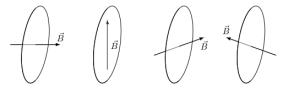
\includegraphics[scale=1]{indquali_c}
	      %     \label{fig:indquali_c}
	      %   \end{figure}
\end{enumerate}

\section{Spire en rotation}
\label{sec:spirerot}

\noindent
\begin{minipage}[t]{.6\linewidth}
	On considère une spire conductrice circulaire de surface $S$ et de résistance
	électrique $r$. Cette spire est mise en rotation à la vitesse angulaire $\Omega
		= \dot{\tt}$ constante autour d'un de ses diamètres, qui définit l'axe
	$\Delta{}$ (cf.\ figures en perspectives ci-contre). Elle est placée dans un
	champ magnétique uniforme et stationnaire $\vv{B}$ orthogonal à $\Delta{}$.
	\begin{enumerate}
		\item Établir l'expression de la f.é.m.\ induite dans la spire. En déduire
		      celle du courant induit dans la spire.
	\end{enumerate}
\end{minipage}
\hfill
\begin{minipage}[t]{.39\linewidth}
	~
	\vspace{-10pt}
	\begin{center}
		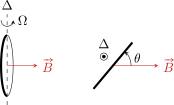
\includegraphics[scale=1]{spirot}
		\label{fig:spirot}
	\end{center}
\end{minipage}

\begin{enumerate}[start=2]
	\item Déterminer le moment magnétique instantané (dépendant de $t$) de la spire.
	\item En déduire le couple de \textsc{Laplace} instantané puis moyen qui
	      s'exerce sur la spire. Quel est qualitativement son effet sur le mouvement
	      de la spire~? Aurait-on pu le prévoir sans calcul~?
\end{enumerate}

\section{Mesure d'une inductance mutuelle}
\label{sec:mesindmut}

\noindent
\begin{minipage}[t]{.6\linewidth}
	Le montage ci-contre permet de mesurer le coefficient d'inductance mutuelle
	entre deux bobines. Les deux bobines se font face comme sur la figure
	ci-contre. La première bobine est montées en série avec une résistance $R =
		\SI{100}{\Omega}$ et un générateur de tension $e_0$ harmonique de fréquence $f
		= \SI{2.0}{kHz}$. Les tensions $u_1$ et $u_2$ sont mesurées grâce à un
	oscilloscope supposé idéal, c'est-à-dire de résistance d'entrée infinie.
\end{minipage}
\hfill
\begin{minipage}[t]{.39\linewidth}
	~
	\vspace{-10pt}
	\begin{center}
		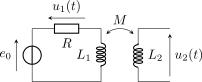
\includegraphics[scale=1]{indmut}
		\label{fig:mesindmut}
	\end{center}
\end{minipage}

\begin{enumerate}
	\item Quelle est l'intensité circulant dans la bobine 2~? D'après la loi de
	      comportement habituelle de la bobine, que vaudrait alors la tension $u_2$~?
	      Pourquoi cette n'est-elle pas applicable telle quelle ici~?
	\item Exprimer la tension $u_2$ en fonction de $M$ et $u_1$.
	\item Calculer $M$ en sachant que les tensions lues à l'oscilloscope ont des
	      amplitudes $U_1 = \SI{3.00}{V}$ et $U_2 = \SI{0.5}{V}$.
	\item On fait tourner la bobine sur elle-même dans le plan de la paillasse.
	      Indiquer sans calcul comment est modifiée la valeur de $M$ lorsque l'angle
	      de rotation vaut $\ang{180}$, et $\ang{90}$. Même question si on aligne les
	      axes des deux bobines.
\end{enumerate}

\section{Solénoïdes imbriqués}
\label{sec:solimb}
Deux solénoïdes $\Sr_1$ et $\Sr_2$ de même axe $(\Or z)$, de même longueur $\ell
$ et de rayons $r_1$ et $r_2 > r_1$ sont emboîtés l'un dans l'autre, comme
représenté Figure~\ref{fig:solimb}. Ils possèdent tous deux le même nombre de
spires $N$. On suppose que la longueur $\ell $ est très supérieure aux rayons.
\begin{figure}[h]
	\centering
	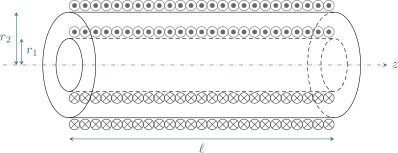
\includegraphics[scale=1]{solimb}
	\caption{Solénoïdes imbriqués.}
	\label{fig:solimb}
\end{figure}
La bobine intérieure est parcourue par un courant $i_1(t) = I \cos{\wt}$ avec $I
	= \SI{1}{A}$. La bobine extérieure est en court-circuit.
\begin{enumerate}
	\item Déterminer les coefficients d'induction propre $L_1$ et $L_2$, ainsi que
	      le coefficient d'induction mutuelle $M$.
	\item En négligeant les résistances internes des fils, déterminer le courant
	      $i_2(t)$ parcourant la bobine extérieure. Quelle est son amplitude~?
	\item Que vaut le champ magnétique à l'intérieur du solénoïde central~?
\end{enumerate}

\section{Plaque de cuisson à induction}
\label{sec:plqind}
Le chauffage du fond métallique des casseroles et autres poêles de cuisson peut
être réalisé par effet \textsc{Joule} des courants induits directement dans le
fond de la casserole par un champ magnétique variable, appelés \textit{courants
	de \textsc{Foucault}}.

\begin{itemize}[label=$\diamond$, leftmargin=10pt]
	\item Logé dans une table support en céramique, un bobinage alimenté en
	      courant sinusoïdal (appelé \ul{inducteur}) génère ce champ. L'inducteur a un
	      rayon de \SI{5}{cm} et compte \SI{20}{spires} de cuivre de résistance
	      électrique $R_1 = \SI{18}{m\Omega}$ et d'auto-inductance $L_1 =
		      \SI{30}{\micro H}$. Il est alimenté par une tension harmonique $v_1$ de
	      pulsation $\w$.
	\item Du point de vue électromagnétique, on modélise le fond de la casserole
	      par une spire circulaire unique, fermée sur elle-même, appelée \ul{induit}.
	      L'induit a une résistance $R_2 = \SI{8.3}{m\Omega}$ et une auto-inductance
	      $L_2 = \SI{0.24}{\micro H}$.
	\item Le transfert d'énergie électrique s'effectue par un couplage inductif
	      entre l'inducteur et l'induit d'inductance mutuelle $M = \SI{2}{\micro H}$.
\end{itemize}

\begin{enumerate}
	\item En s'appuyant sur un schéma électrique équivalent, établir les équations
	      électriques relatives aux deux circuits.
	\item En déduire l'expression littérale de la fonction de transfert $\ul{H} =
		      \frac{\ul{I_2}}{\ul{I_1}}$.
	\item En déduire l'impédance d'entrée $\ul{Z_e} = \frac{\ul{V_1}}{\ul{I_1}}$
	      du système.
	\item La pulsation $\w$ est choisie bien plus grande que $R_1/L_1$ et
	      $R_2/L_2$, avec $\w = \SI{7.0e4}{rad.s^{-1}}$. Simplifier les deux
	      expressions précédentes et calculer numériquement leur module.
	\item On soulève la casserole. Indiquer qualitativement comment varie
	      l'amplitude du courant appelé par l'inducteur.
\end{enumerate}

\section{Peut-on négliger l'auto-induction~?}
\label{sec:neglautoind}

\noindent
\begin{minipage}[t]{.6\linewidth}
	On fait très souvent l'approximation de négliger l'auto-induction dans les
	circuits ne comportant aucun bobinage. On s'intéresse dans cet exercice à la
	validité de cette approximation pour un circuit \textit{a priori} quelconque,
	schématisé ci-contre, d'auto-inductance $L$. Le circuit, de surface totale $S$
	et de résistance $R$, est plongé dans un champ magnétique extérieur $\vv{B}_{\rm
			ext} = B_0 \cos{\wt}\vv{n}$.
\end{minipage}
\hfill
\begin{minipage}[t]{.39\linewidth}
	~
	\vspace{-10pt}
	\begin{center}
		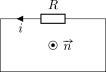
\includegraphics[scale=1]{autoindnegl}
		\label{fig:autoindnegl}
	\end{center}
\end{minipage}

\begin{enumerate}
	\item Commençons par ne prendre en compte que la f.é.m.\ induite par le champ
	      $\vv{B}_{\ext}$. Calculer son flux au travers du circuit, et en déduire la
	      schéma électrique équivalent. Que vaut l'intensité $i$~?
	\item Considérons en plus le phénomène d'auto-induction. Exprimer le flux
	      magnétique au travers du circuit et représenter le schéma électrique
	      équivalent. Établir l'équation différentielle vérifiée par $i$.
	\item Passons maintenant en notation complexe. Exprimer le rapport $\abs{H} =
		      \abs{\ul{E}_L}/\abs{\ul{E}_{\ext}}$ des amplitudes de la f.é.m.\
	      auto-induite et de la f.é.m.\ induite par le champ extérieur. En déduire à
	      quelle condition sur la pulsation la f.é.m.\ auto-induite est négligeable
	      devant la f.é.m.\ induite.
	\item Pour fixer les idées, calculer numériquement la pulsation et la
	      fréquence caractéristiques avec des valeurs de $R$ et $L$ utilisées
	      habituellement en TP d'électrocinétique. Quel résultat connu retrouve-t-on~?
	\item En proposant des ordres de grandeur raisonnables, refaire le même calcul
	      pour un circuit de même résistance mais à une seule «~spire~» composée d'un
	      fil de cuivre de TP. L'inductance d'un circuit circulaire de diamètre $D$ et
	      donnée par
	      \[
		      L = \mu_0 \frac{D}{2} \left( \ln \frac{8D}{d} - 2 \right)
	      \]
	      où $d$ est le diamètre du fil de cuivre. Est-il légitime de négliger
	      l'inductance du circuit~?
\end{enumerate}

\section{Principe de fonctionnement d'un générateur synchrone}
\label{sec:motsynch}
\noindent
\begin{minipage}[t]{.6\linewidth}
	Un aimant de moment magnétique $\vv{m_0}$ est placé dans le plan $(\Or xy)$. Un
	système mécanique le met en rotation à vitesse angulaire $\w$ constante autour
	de l'axe $(\Or z)$. Un spire circulaire de rayon $a$ et de résistance $R$ est
	placée sur l'axe $(\Or x)$ à distance $x \gg a$.
\end{minipage}
\hfill
\begin{minipage}[t]{.39\linewidth}
	~
	\vspace{-20pt}
	\begin{center}
		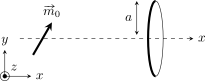
\includegraphics[scale=1]{motsynch}
		\label{fig:motsynch}
	\end{center}
\end{minipage}

\begin{tdefi}{Donnée}
	En coordonnées polaires d'axe colinéaire à $\vv{m}$, un moment magnétique
	$\vv{m}$ placé à l'origine créé en un point M quelconque un champ magnétique
	\[
		\vv{B}(\Mr) = \frac{\mu_0 m}{4\pi r^3} (2 \cos{\theta}\ur + \sin{\theta} \ut)
	\]
\end{tdefi}
\begin{enumerate}
	\item Déterminer l'intensité $i$ du courant induit dans la spire. En déduire
	      la puissance électrique qu'elle reçoit. Une attention particulière sera
	      donnée à l'orientation de l'angle $\tt$, et on vérifiera qualitativement les
	      signes de la f.é.m.\ et du courant induits.
	\item Exprimer le couple magnétique subi par l'aimant \textbf{de la part de la
		      spire}. On fera attention au point d'origine du champ magnétique que subit
	      l'aimant, et on vérifiera encore les signes obtenus.
	\item Quelle puissance le système mécanique doit-il fournir à l'aimant pour le
	      maintenir à vitesse constante~? Conclure~: en quoi a-t-on modélisé un
	      générateur électrique rudimentaire~?
\end{enumerate}


\end{document}
